\chapter{Introduction}
\section{Nuclear matter under extreme conditions}
The quest for the matter and its properties under extreme highly density and temperature has fundamental importance.
Understanding nuclear matter and under these conditions help to understand questions from the early dynamics of the universe to the neutron star merger simulation for the gravitational wave studies.
It also help to enrich the understanding of the fundamental theory of the strong interaction and basics to the nuclear physics: the Quantum Chromodynamics (QCD).

\paragraph{Quantum Chromodynamics}
QCD describes the interaction of objects that carries ``color'' charges.
Quarks (fermions) and gluons (bosons) are its elementary degrees of freedom. 
The QCD Lagrangian (with one flavor of quark) is,
\begin{eqnarray}
\mathcal{L} = \bar{\psi_i} \left(i\gamma_\mu D^\mu_{ij} -m \delta_{ij} \right)\psi_j - \frac{1}{4}G_{\mu\nu}^a G^{\mu\nu,a},
\end{eqnarray}
where $\psi_i$ the Dirac spinor of the quark field with $i$ the color index.
\begin{eqnarray}
D_{ij}^\mu = \partial^\mu - i g T_{ij}^a A^{\mu, a}
\end{eqnarray}
is the covariant derivative, containing the interaction between quark field and the gluon field with coupling strength $g$.
Here $T_{ij}^a$ are the generators of the SU(3) group in the fundamental representation and the generators satisfies the commutation relation,
\begin{eqnarray}
[T^a, T^b] = i f^{abc} T^c
\end{eqnarray}
where $f^{abc}$ are known as the structure constants of SU(3).
The field tensor of gluon with color $a$ is,
\begin{eqnarray}
G^{\mu\nu,a} = \partial^\mu A^{\nu, a} - \partial^\nu A^{\mu, a} + g f^{abc} A^{\mu,b}A^{\mu,c}
\end{eqnarray}
The first term is the kinetic term, and the second term is the gluon field self-interation (also with strength $g$) is a unique feature of the non-Abelian gauge field.

\paragraph{Asymptotic freedom and confinement}
Due to quantum fluctuations, the effective coupling constant $g$ changes with the energy scale of a process. 
The rate of change of $g$ with respect to the scale parameter is called the $\beta$-function,
\begin{eqnarray}
\frac{\partial g}{\partial \ln\mu} = \beta(g),
\end{eqnarray}
which can be evaluated as a perturbation series of $g$.
At leading order, the QCD $\beta$ function with number of colors $N_c$ and $n_f$ flavors of fermion is,
\begin{eqnarray}
\beta(g) = - \left( \frac{11}{3}N_c - \frac{2}{3}n_f \right) \frac{g^3}{16\pi^2}.
\end{eqnarray}
This $\beta$ function is negative for QCD ($N_c=3$) using realistic numbers of quark flavors $n_f = 2\cdots 6$, meaning the effective coupling constant decreases with increasing energy scale.
The property is known as the asymptotic freedom of QCD because the interaction becomes small at asymptotically high energy, which also makes possible the use of perturbation theory at high energy.

Often a strong coupling constant is defined as $\alpha_s = g^2/4\pi$.
Using the leading order $\beta$-function, its scale dependence is
\begin{eqnarray}
    \alpha_s(Q^2) = \frac{4\pi}{\left(\frac{11}{3}N_c - \frac{2}{3}n_f\right)\ln\left(\frac{Q^2}{\Lambda^2}\right)}.
\end{eqnarray}
The integration constant has been absorbed into the QCD scale parameter $\Lambda$.
Therefore, at least in perturbation theory, $\Lambda$ becomes the only parameter of QCD. 
Its value is determined by anchoring $\alpha_s(\mu)$ to the experimental measurement at a fixed scale, for example, $\alpha_s(M_z) = 0.1185$ at the scale equal to the $Z$ boson mass.
The leading order $\Lambda$ is then around $200$ MeV.

The decreasing of $\alpha_s(Q)$ is logarithmic slow at high energy, but it rises quickly approaching with $Q$ approaching $\Lambda$ from above.
Even before reaching this scale, the coupling constant is already too large for a reliable perturbative calculation.
Near the $\Lambda$ scale, QCD enters the non-perturbative region,
and at this long distances only hadrons exists as colorless bound states of quarks and gluons.
The fact that colors not directly observed at large distances is knowns as ``color confinement'' of QCD. 
To pull a quark out of the hadron, the color field becomes so strong that eventually more quark-anti-quark pairs populated in-between the pulled quark and the remnant and forms new colorless hadrons.

Depending on its valance quarks (quarks that carry the net quantum number of the hadron) content, hadrons are generally categorized as baryons and mesons.
Baryon has three valance quarks or anti-quarks, such as neutrons and protons.
Meson has a valance quark and an anti-quark, such as pion and kaon.
Hadrons are also populated with sea-quarks and gluons that are constantly produced and annihilated as quantum fluctuations.
The momentum of hadron is mostly carried by the valance quarks.
The sea quarks and gluons together share the rest fraction of the total momentum, but their abundance number at high energy is very important for the particle production in relativistic hadron / heavy-ion collisions.

Nowadays, the only reliable ab initio theoretical tool for non-perturbative QCD is lattice field theory technique, where the QCD Lagrangian is discretized on a finite lattice and studied on a computer.

\paragraph{The phase-diagram of the QCD matter}
At zero temperature ($T$), protons and neutrons (together as nucleons) form bound states of atomi nuclei that build the ordinary matter.
One can also define the baryon chemical potential $\mu_b$, and for ordinary matter $\mu_b$ is around $1$ GeV, close to the proton mass.
The ordinary nuclei is indicated as the white dot on the (partly conjectured) phase diagram in figure \ref{fig:phase-diagram} [].
Increasing the temperature of the system, nucleons start escape from nuclear potential and other hadrons can be created from collision and resonance formation and decay.
This system is know as the hadron gas (cyan region in figure \ref{fig:phase-diagram}).

Because QCD has asymptotic freedom at high energy and confinement at low energy scale, there can be so-called deconfinement phase-transition when temperatures crosses the QCD non-perturbative scale.
At asymptotically high temperature, the weakening of the coupling should lead to the transit from the color confined hadronic matter to a system of transporting quarks and gluons, termed the quark-gluon plasma (QGP). 
Frist principle lattice QCD calculations have studied this transition at zero baryon chemical potential with 2+1 flavors (up / down plus strange quark) QCD.
Figure \ref{fig:qcd_eos} quotes the equation of state computed by  the HotQCD Collaboration [].
It shows the pressure $P$, energy density ($\epsilon$) and entropy density ($s$) of QCD system.
These thermodynamic quantities are scaled by powers of temperature, so that the ratio can be loosely related the effective number of degrees of freedom (DoF) of the system
The Stefan-Boltzmann limit (non-interacting gas of quarks and gluons) is denoted as the dashed lines in the up-right corner.
It is observed that the effective number of DoF converges to the expectation from a hadron resonance gas model (solid lines) at low temperature and rapidly increases to a value close to the Stefan-Boltzmann limit in a narrow temperature window.
This suggests a releasing of the quark and gluon degrees of freedom at high temperature.
More close study indicate that this is not a real phase-transition at ($\mu_b = 0$), and sometimes people also refer to it as a ``cross-over'' phase transition, where the thermaldynamical quantity is smooth across this region of phase-diagram.
Nevertheless, a pseudo critical temperature is defined to be $T_c \approx 150 $ MeV, corresponding to 1.5 trillion Kelvin.

\begin{figure}
    \centering
    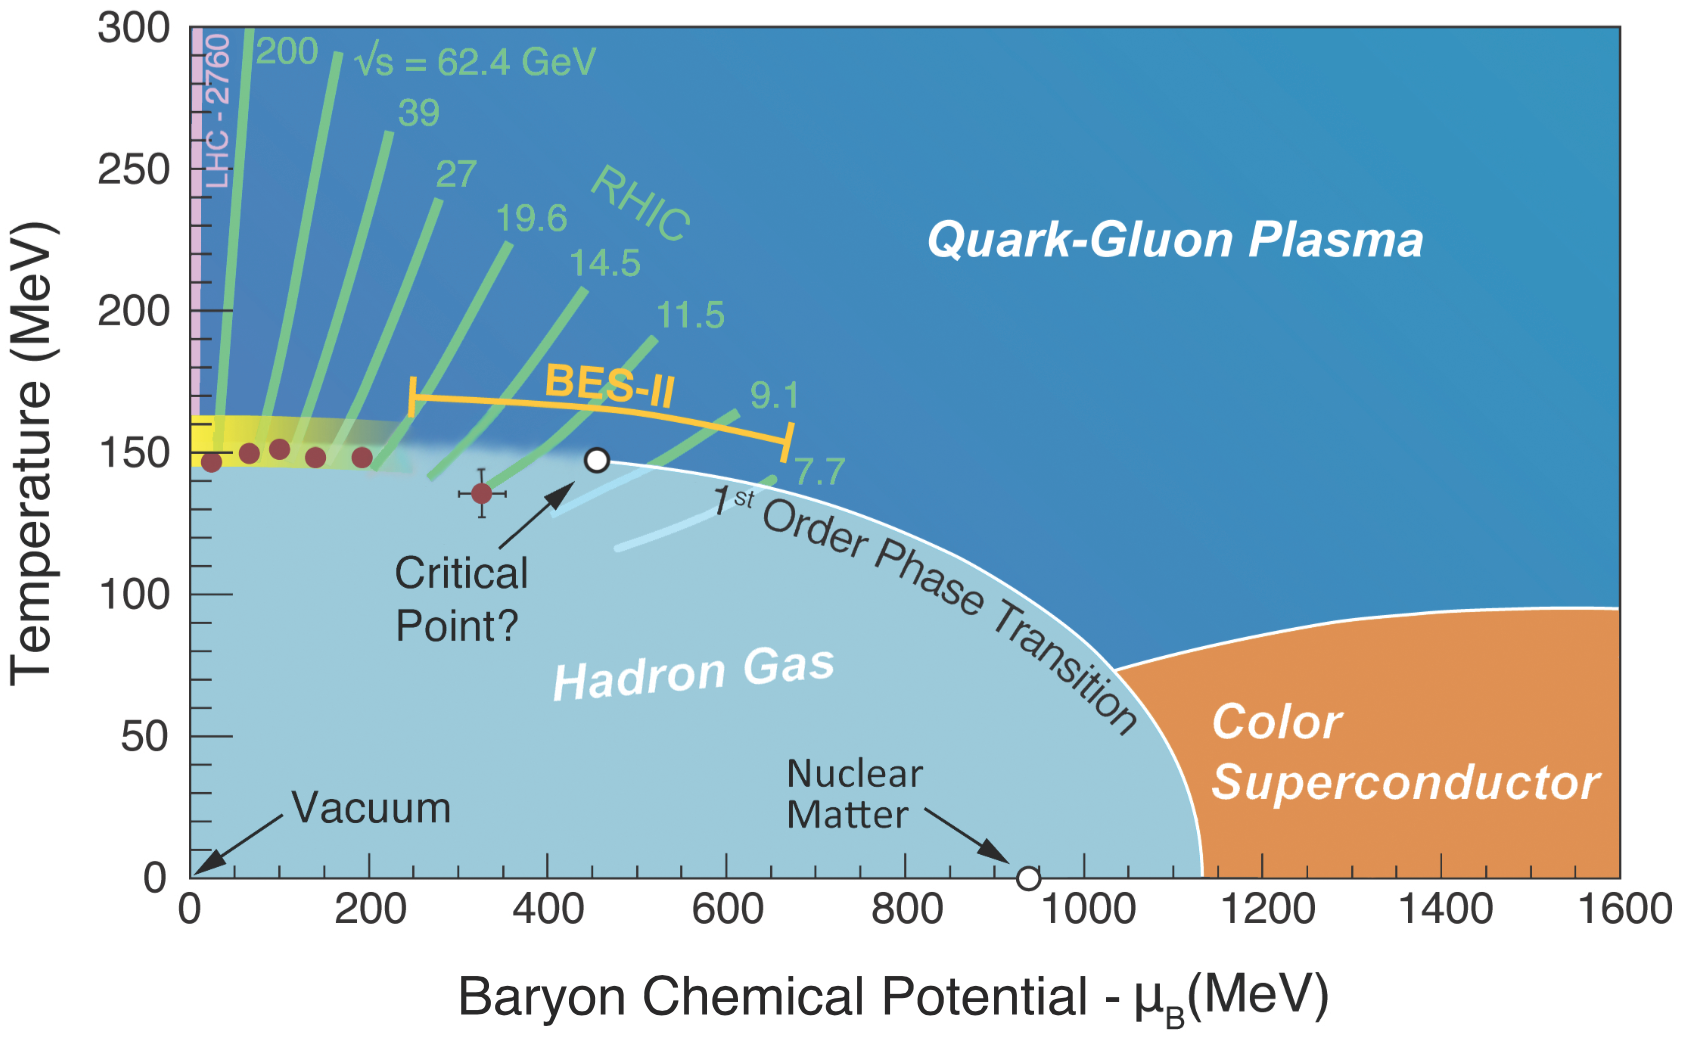
\includegraphics[width=.8\textwidth]{phase-diagram.png}
    \caption{Caption}
    \label{fig:phase-diagram}
\end{figure}

Moving to wards finite baryon chemical potential, the lattice approach runs into the fermion sign problem, though recent studies has been pushing the realm of lattice QCD into small $\mu/T$ regions [].
Effective models [] and Dyson-Schwinger equation studies [] have suggested the existence of a first order phase transition at large $\mu_B/T$.
If true, the first-order coexistence line must end at a point on the phase-diagram at lower $\mu_b$, beyond which the phase-transition is the cross-over type.
Such a point, called the critical end point (CEP), has attached a great interest of both theoretical confirmation / exclusion and experimental search.

At higher chemical potential and low temperature, another phase of nuclear matter known as the ``color superconducting phase'' is proposed, where the quarks forms Cooper pairs in analogy to the superconductors [].

\begin{figure}
    \centering
    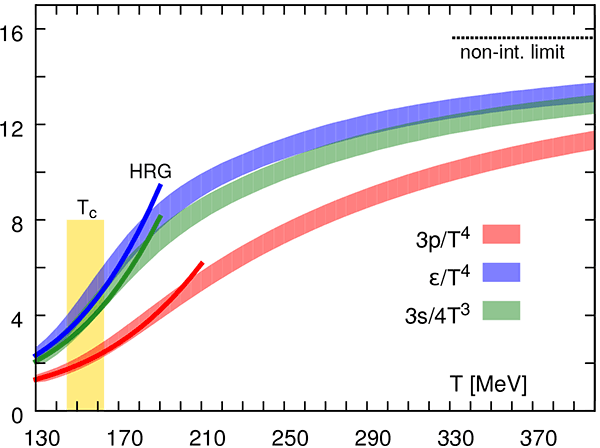
\includegraphics[width=.8\textwidth]{qcd-eos.png}
    \caption{Caption}
    \label{fig:qcd_eos}
\end{figure}

It is believed that the QCD high-temperature phase-transition is a stage of the universe around a microsecond after ``the Big Bang'', when the temperature drops down to QCD scale.
Compact starts are ``celestial laboratories'' to test the QCD equation-of-state in the high density and low temperature region, providing an important physical input for simulating the recently discovered gravitational wave from neutron star mergers.
In laboratories, we create hot and dense nuclear matter by colliding heavy nuclei at ultra-relativistic high energies.
Though the created matter is so transient and tiny compared to the cosmic nuclear matter, we can learn not only thermodynamic properties but also essential dynamical properties of the QCD in these experiments.

\section{Phenomenology of relativistic heavy-ion collision}
Relativistic heavy-ion collision is currently the only tool to access high energy density QCD medium in laboratory.
Since 2005, the Relativistic Heavy-ion Collider (RHIC) at the Brookheaven National Laboratory (BNL) started colliding gold nuclei at 200 GeV []. 
The Large Hadron Collider (LHC) started its heavy ion programs later, colliding lead nuclei at 2.76 TeV and 5.02 TeV [].
Since then, many evidences have been pointing to the discovery of the new state-of-matter: the strongly coupled quark-gluon plasma (sQGP).
In this section, I shall introduce useful concepts and terminology in heavy-ion collisions.
Then I will review a few important experimental evidences and how they can help the understanding of the properties of the sQGP.

\subsection{Nuclear collisions geometry}
\paragraph{Kinematics} For the case of ultra relativistic collisions, it is advantages to use a new set of coordinates that is related to the Cartesian coordinates by,
\begin{eqnarray}
x_\perp &=& x_\perp\\
\tau &=& \sqrt{t^2 - z^2}\\
\eta_s &=& \frac{1}{2}\ln\frac{t+z}{t-z}
\end{eqnarray}
where the $z$ direction aligns with the accelerated beam direction.
$\tau$ is called the ``proper time" and $\eta_s$ called the space-time rapidity.
One advantage of using this set of coordinates is that $\tau$ and $\eta_s$ transforms much simpler than $t$ and $z$ under Lorentz boost ($\beta_z$) in the beam direction,
\begin{eqnarray}
\tau' &=& \tau,\\
\eta_s' &=& \eta_s + \frac{1}{2}\ln\frac{1+\beta_z}{1-\beta_z}
\end{eqnarray}
Similarly for momentum, the four components of $p^\mu$ can be transformed into,
\begin{eqnarray}
p_\perp &=& p_\perp\\
m_T &=& \sqrt{E^2 - p_z^2}\\
y &=& \frac{1}{2}\ln\frac{E+p_z}{E-p_z}
\end{eqnarray}
where $m_T$ is called transverse mass, and $y$ the rapidity of a particle.
Besides, pseudorapidity is often used experimentally,
\begin{equation}
\eta = \frac{1}{2}\ln\frac{|p|+p_z}{|p|-p_z} = \frac{1}{2}\ln\frac{1+\cos\theta}{1-\cos\theta}
\end{equation}
It has the merits that it is directly related to the polar angle of final state particles.
When the transverse mass is small compared to $p_z$, the pseudorapidity is also a good proxy of rapidity.

\paragraph{Centrality as a geometry handle of nuclear collisions}
Nuclei are extended objects.
The heavy nuclei radius is approximately scales like $A^{1/3}$ fm, where  $A$ is the atomic number. 
For example, the the radius of a gold and a lead nuclei is about $6-7$ fm upto some diffuseness in the boundary.
In the center-of-mass frame,  nuclei ``shrink" in the $z$ direction by the factor $\gamma = (1-v^2)^{-1/2} = E/M$ because of the Lorentz contraction.
$\gamma$ is a large number, it is over $100$ for gold nuclei at top RHIC energy can be $2500$ for lead nuclei at the LHC.
Therefore, the tow nuclei contracted into thin `pancakes` while approaching each other.

Defining the impact parameter $\vec{b}$ as the transverse separation between the center-of-mass of the two approach nuclei,
the geometry of the collisions can therefore fluctuate from a completely overlapping one ($b=0$) to very peripheral interaction (large $b \gtrsim 2R$).
We will see later that the geometry of a collision event is a useful handle to study the property of its dynamical evolution, however, it is impossible perform high energy experiments with only certain ranges of the impact parameter. 
What is used as an approximate collision geometry indicator in nuclear-nuclear collisions is the so-called centrality.
Centrality can be defined in different ways (multiplicity / transverse energy) and with different kinematic cuts, but the idea is to reflect the nuclear collision geometry by particle production activity.
It is reasonable to anticipate that the average number of charged particles produced or the total transverse energy deposited within a certainty detector acceptance are higher if the collision is more central (small impact parameter), and are lower for peripheral collision.
The relation between centrality and geometry is not exact, because fluctuation in particle production smears out one-to-one correspondence between the impact parameter an the ``centrality meter''.

Experimentally, a minimum-biased sample of recorded events are sorted according to the centrality criteria (multiplicity, e.g.) and the events are binned by percentile.
Then, for example, the top 0--5\% highest multiplicity events are associated to the central collisions with centrality range 0--5\% through a model.
Usually, the models is one of the many variants of the Monte-Carlo Glauber model (to be explained in section \ref{simulation}), which samples the  number of binary nucleon-nucleon collisions and number of participants (nucleons that suffers at least one binary collisions) at a given impact parameter.
It is found that the bulk particle production scales roughly like number of participants, while the cross-section of hard processes (processes involves large momentum transfer $Q \gg \Lambda$).
It is true that the centrality definition can be model dependent, but the uncertainty can be quantified and its prediction can be validated by the production of colorless probes.

\subsection{Particle production mechanisms}
Experimentally, it is found that the particle produced in relativisitc nuclear collisions has a wide pseudo-rapidity distribution, and a steep falling transverse momentum spectra.
The bulk of the particles in one event are relatively soft with $p_T \lesssim 3$ GeV.
One of the most striking discovery from RHIC and LHC heavy-ion program is that these soft particles depicts a strong collectivity, and hydrodynamic based models are able to describe the bulk observables to a very high precision.
This success of the hydrodynamic model reveals the strongly coupled nature of the matter produced with a temperature several times above $T_c$ and it has been entitled the name strongly coupled quark-gluon plasma (sQGP).
This is in contrary to the previous expectation of a weakly coupled gas of quarks and gluons.

\subsection{Anisotropic flow and QGP transport coefficient} 
One of the manifestation of collectivity is the momentum space anisotropy of the final state. 
Decomposing the charged particle spectra into Fourier series of the azimuthal angle,
\begin{eqnarray}
E\frac{dN}{p_T dp_T d\phi dy} = \frac{1}{2\pi}\frac{dN}{p_T dp_T dy}\left(1 + \sum_{n=1}^{\infty}v_n(p_T)\cos\left[n(\phi-\Psi_n)\right]\right).
\end{eqnarray}
The first term in the expansion is azimuthal angle averaged yield.
The terms in the sum expands the angular dependence. 
The $n=1$ term is a movement of the center-of-mass.
From $n=2$, a non-zero $v_n$ characterize the anisotropy in momentum-space of various order.
If the particle production in high energy nuclear collisions is simply an independent sum of elementary nucleon binary collisions, then the anisotropy would be zero after averaging over many events. 
However, experiments observe a surprisingly larger elliptic flow ($v_2$) in Au+Au collisions and later in Pb+Pb collisions.
Higher order flows harmonics and in particular odd order $v_n$ were observed later.
The large anisotropic flow suggests a substantial role of final state interaction after the initial production.
In the hydrodynamic picture, non-central collisions results in an initial almond shape of the deposited energy density and the hydrodynamic pressure builds up and drives the transverse expansion of the fireball.
Because the pressure gradient is larger in the short axis-direction and the long-axis direction, the matter flows in an isotropic way, creating the observed momentum space anisotropy.
Higher order of flow harmonics is a result of the initial state fluctuation of the nuclear wave function.
In short, the hydrodynamics transfer initial geometry eccentricities $\epsilon_n$ into final state momentum anisotropy $v_n$.

A relativistic ideal hydrodynamic model (no viscous effect) assumes an infinitely strong interaction that the medium always stages in local thermal equilibrium.
A more realistic system with finite interact strength will go off-equilibrium under the driven force, and is treated in relativistic viscous hydrodynamics with shear viscosity $\eta$ and bulk viscosity $\zeta$ as inputs.
Because the viscous effects damp the spatial anisotopic of the flow, the efficiency of the transition from $\epsilon_n$ to $v_n$ is very sensitive to the values of shear and bulk viscosity and can be used for precision extraction of the these number from experimental measurements.

The QGP shear viscosity and bulk viscosity are of fundamental importance. 
The shear viscosity to entropy ratio $\eta/s$ is an indicator of the stong / weak coupling nature of the QGP. 
And the bulk viscosity to entropy ratio $\zeta/s$ is directly related to  the scale-invariance breaking of QCD.
Dynamical quantities such as viscosity are extremely hard to be computed from first principle, so currently, pinning down these numbers and their temperature / chemical potential dependences from experiments is essential in learning the dynamical properties of QGP.
Global comparisons of the state-of-the-art medium modeling to a collection of soft observables have corroborate the need of a small $\eta/s$ that are likely to be slowly increasing with temperature and a non-vanishing $\zeta/s$.

\subsection{Constituent quark scaling and the degrees freedom}
The hydrodynamics is successful on describing the collectivity, but does not assume what is the effective degrees of freedom that is flowing.


\subsection{Probing sQGP with hard probes}
Very occasionally, particles with large transverse momentum ($p_T\gtrsim 10$ GeV) are produced, and there are referred to as the ``hard" particles.
By uncertainty principal, these hard particles can only be produced in the initial collisions on a time scale $\delta t \sim 1/p_T$.
Therefore, a hard process can only be produced at the very beginning of the nuclear collision and interacts with the nuclear medium that surrounds it.
Due to the large $p_T$ and relatively small coupling constant, the production of these hard particles can be studied in a perturbative framework.
The interaction with the medium modifies the initial production and leaves finger prints of the nuclear matter properties in the hard observables. 
So, these hard particles can be used as self-generated probes of the system.

\paragraph{Jet and jet quenching}
Jet quenching refers to the strong suppression of the yield of high transverse momentum hadrons in nuclear collisions, compared to the scaled yield in proton-proton collisions where medium effects are assumed to be small.
Calculations have shown that this suppression is a consequence of jets losing energy to the hot, dense and color-deconfined medium. 

\paragraph{Heavy-flavor probes}
Heavy quarks (charm and bottom) are often seen as complementary probes of the QGP, but partly also belong to the category of jet observables, depending on their transverse momenta. Their large masses (compared to the prevailing temperatures generated in collisions at current heavy-ion colliders) constrain their production to early reaction times via hard perturbative Quantum-Chromodynamics (pQCD) processes. Flavor conservation ensures that the overwhelming majority of heavy quarks survive the entire reaction, allowing them to probe the full space-time evolution of the reaction.
These two features are particular attractive to theorists as these flavor-tagged particles are much easier to track in the calculations than the evolution of a full jet.
The mass also sets an additional energy scale to the problem and brings rich physics to the heavy-flavor sector.
In the high transverse momentum region, heavy quarks lose energy mainly through radiative processes connecting them to jet energy loss studies {Wicks:2007am, Djordjevic:2004nq, Xu:2014tda, Kang:2016ofv}, whereas
in the low transverse momentum region their large mass delays their thermalization, providing a window to study the equilibration process {Moore:2004tg,Riek:2010fk,Cao:2013ita}.
Heavy flavors are therefore ideal and unique probes to determine QGP properties.

The in-medium propagation of heavy quarks is often studied in a kinetic approach that is linearized with respect to the heavy quark distribution function and the medium particle distribution function is assumed to be thermal, obtained from hydrodynamic models.
The linearization implies that any effects of the heavy quark interactions on the medium are neglected.

The linearized Boltzmann transport equation and the Langevin equation are both widely used linearized models but make different assumptions regarding the nature of the interaction and thus often focus on different regimes in the heavy quark phase space {Auvinen:2009qm,Cao:2016gvr, Cao:2017hhk, PhysRevD.37.2484, Moore:2004tg}.
The linearized Boltzmann transport equation is based on elementary scattering processes that can be directly calculated, e.g. via pQCD.
However, calculations in the presence of a medium are extremely complicated even at leading order {Arnold:2002zm}.
Also, the pQCD processes are often plagued by soft divergences that need to be regulated by a medium scale proportional to temperature. Moreover, at current collision energies the relevant temperature is not high enough which creates ambiguities for the pQCD calculation through the scale dependence of the strong coupling constant $\alpha_s$.

The Langevin equation takes a different approach: 
it assumes that heavy quark receives frequent but soft momentum kicks from the medium, making a statistical description of the interaction possible -- in terms of ``drag" and ``diffusion" coefficients.
These transport coefficients encode the first and second moments of the momentum-exchange rate but are agnostic to further details of the elementary processes and medium properties.
There are efforts to calculate these transport coefficients in various approaches including lattice QCD {Moore:2004tg,CaronHuot:2008uh, Gossiaux:2008jv,He:2012df,Riek:2010fk,vanHees:2007me,Scardina:2017ipo,Ding:2012sp,Banerjee:2011ra,Francis:2015daa}. Our group has taken a complementary approach, using experiment data to calibrate our Langevin based transport model to measured observables and thus extract the transport coefficients directly from data via a Bayesian analysis {Xu:2017obm}. The drawback of this approach is that it does not in itself provide a fundamental understanding of the interaction mechanism but can only provide guidance to direct calculations of the transport coefficients in terms of compatibility to experimental observation.

\section{Extract sQGP properties from model-to-data comparison}
Immediately after the nuclei penetration through each other $t\sim 2R/\gamma$, huge amount of energy is deposited into the overlapped area and entropy is produced, creating a fireball in the middle while the nuclear remnants recede.
This highly excited fireball of fields undergoes complex dynamics and cools down rapidly because of the longitudinal and transverse expansion.
Eventually, it reaches to a point where the temperature is low enought that the quarks and gluons are again confined into hadrons. 
The hadrons can have further interactions and may decay into other hadrons, photons and lepton.
The dynamical of QGP we are interested in only lasts for $O(10) fm/$c, while we can only observe the remnants at the end of the collisions.
Therefore, the understanding of the QGP requires both an accurate dynamical modeling of the entire process and the design of sensitive observables.


\paragraph{Complex dynamical model with high-dimensional inputs}
Taking the bulk model as an example, it includes an initial condition, a dynamical model for pre-equilibrium stage, the viscous hydrodynamics, particlization of the hydrodynamic energy momentum tensor and the hadronic decays and rescatterings.
Each of the module takes both physical parameters and modeling parameters.
Eventually, one can have more than 10 parameters.
To generate one event with a model itself is already computationally intensive, while to be able to compare to experimental measurements that average over centrality with a good control of statistical uncertainty, $O(10^4)$ minimum-biased events needed to be generated.
As a result, a na\"ive linear grid sweep over the 10-dimensional parameter space is certainty not feasible.
To solve this problem of high-dimensional input complex models requires advanced parameter set design method and reliable interpolation schemes.


\paragraph{Model uncertainty and correlation among parameters}
We are mostly interested in those ``physical parameters / quantities'', for example, the transport coefficients $\eta/s(T)$ and $\zeta/s(T)$ of the medium.
Other parameters, such the switching time between the pre-equilibrium free-streaming dynamics and the hydrodynamics, and the temperature at which one particlize a hydrodynamic field description into a hadronic ensemble are less interested in the physical sense.
The appearance of these matching parameters are simply due to we do not have a single ``global model'' that works reasonably well under all circumstances.
However, one should not think less of these model parameters, because the quantify a significant fraction of the modeling uncertainty.
The model uncertainty can affect the interpretation of the experimental data, and any quantitative statement we draw about those physical quantities from a model-to-data comparison.
For example, the  bulk particles anisotropic flows, though proved to be very sensitive to the shear viscosity, are also sensitive to the initial eccentricity of the initial conditions.
Therefore, the exacted $\eta/s$ becomes correlated with the choice of initial condition models and its parameters.
The model uncertainty is hard problem, and one can either try to reduce it by improving the model or quantify it when compared to data to prevent an over-interpretation.

\paragraph{A high-dimensional model output / observables}
The inclusion of more observables also helps to break the model degeneracy and parameter correlation.
But it can be tricky to quantify the quality of agreement between model and data with a collection of observables (a high dimensional output).


The Bayesian analysis framework is introduced to the field by the earily works of and the PhD thesis of Jonah Bernhard [] who has successfully applied the tool to the extraction of the initial condition topology and temperature dependent QGP transport coefficient.
This chapter provides a concise description of the Bayesian analysis and for full details please refer to the thesis of Jonah Bernhard [].